\chapter{Dasar Teori}
\label{chap:Dasar Teori}

Pada bab ini akan dijelaskan dasar-dasar teori mengenai \textit{library} jsoup meliputi kelas Jsoup, Connection, Response, Document, Elements, dan Element. Selain itu akan dibahas pula mengenai CSS \textit{selector}, Chrome DevTools meliputi panel Elements dan Network, Play Framework, dan SIA Models.

\section{\textit{Library} jsoup}
\label{sec:jsoup}

\textit{Library} jsoup merupakan library Java yang digunakan untuk \cite{jsoup}. jsoup dapat mengambil data berupa HTML dari sebuah situs web. Dalam mengambil HTML, jsoup dapat memanfaatkan \textit{syntax} CSS \textit{Selector} untuk memilih elemen mana saja yang ingin diambil. 

Subbab-subbab berikut menjelaskan beberapa kelas dari jsoup.

\subsection{Jsoup}

Kelas ini merupakan inti untuk mengakses fungsi jsoup. Seluruh \textit{method} dalam kelas ini merupakan \texttt{static} \textit{method} sehingga kelas ini tidak perlu dikonstruksi. Salah satu \textit{method} yang dimiliki kelas ini adalah sebagai berikut:
\begin{itemize}
	\item \textbf{public static Connection connect(String url)} \\
		Berfungsi untuk membuat koneksi baru dengan suatu situs web. \\
		\textbf{Parameter:}
		\begin{itemize}
			\item \textbf{url} URL situs web dengan protokol HTTP atau HTTPS.
		\end{itemize}
		\textbf{Kembalian:} koneksi dengan situs web.
\end{itemize}

\subsection{Connection}

Kelas ini merupakan \texttt{interface} yang menyediakan pengambilan data dari situs web. Beberapa \textit{method} yang dimiliki kelas ini adalah sebagai berikut:

\begin{itemize}
	\item \textbf{Connection cookies(Map<String,String> cookies)} \\
		Berfungsi untuk menambahkan \textit{cookie}. \\
		\textbf{Parameter:}
		\begin{itemize}
			\item \textbf{cookies} \texttt{Map} dari \textit{cookie}.
		\end{itemize}
		\textbf{Kembalian:} koneksi yang sama tetapi sudah diubah.
		
		\item \textbf{Connection data(String key, String value)} \\
		Berfungsi untuk menambahkan parameter data yang bisa dikirim melalui metode HTTP GET atau POST. \\
		\textbf{Parameter:}
		\begin{itemize}
			\item \textbf{key} kunci data.
			\item \textbf{value} nilai data.
		\end{itemize}
		\textbf{Kembalian:} koneksi yang sama tetapi sudah diubah.
		
		\item \textbf{Connection method(Connection.Method method)} \\
		Berfungsi untuk mengatur metode permintaan HTTP, GET atau POST. Metode pengiriman secara \textit{default} adalah GET\\
		\textbf{Parameter:}
		\begin{itemize}
			\item \textbf{method} metode pengiriman permintaan HTTP.
		\end{itemize}
		\textbf{Kembalian:} koneksi yang sama tetapi sudah diubah.
		
		\item \textbf{Connection timeout(int millis)} \\
		Berfungsi untuk mengatur batas waktu \textit{request}. Batas waktu nol akan dianggap sebagai batas waktu yang tak terhingga. \\
		\textbf{Parameter:}
		\begin{itemize}
			\item \textbf{millis} batas waktu dalam milidetik.
		\end{itemize}
		\textbf{Kembalian:} koneksi yang sama tetapi sudah diubah.
		
		\item \textbf{Connection validateTLSCertificates(boolean value)} \\
		Berfungsi untuk mengatur pemeriksaan sertifikat TLS untuk permintaan HTTPS. Nilai \texttt{true} untuk memeriksa dan nilai \texttt{false} untuk tidak memeriksa.\\
		\textbf{Parameter:}
		\begin{itemize}
			\item \textbf{value} status pemeriksaan sertifikat TLS.
		\end{itemize}
		\textbf{Kembalian:} koneksi yang sama tetapi sudah diubah.
		
		\item \textbf{Connection.Response execute()} \\
		Berfungsi untuk mengirim permintaan HTTP.\\
		\textbf{Kembalian:} objek \texttt{Response}.	
\end{itemize}

\subsection{Response}

Kelas ini merepresentasikan permintaan HTTP. Beberapa \textit{method} yang dimiliki kelas ini adalah sebagai berikut:
\begin{itemize}
	\item \textbf{Map<String,String> cookies()} \\
		\textit{Method} ini berfungsi untuk mendapatkan seluruh \textit{cookies}. \\
		\textbf{Kembalian:} seluruh \textit{cookies}.	
		
		\item \textbf{Document parse()} \\
		Berfungsi untuk mengurai \textit{body} jawaban menjadi dokumen. \\
		\textbf{Kembalian:} koneksi yang sama tetapi sudah diubah.
		
		\item \textbf{String body()} \\
		Berfungsi untuk mendapatkan \textit{body} jawaban dalam bentuk \textit{string}. \\
		\textbf{Kembalian:} \textit{body} jawaban dalam bentuk \textit{string}.
\end{itemize}

\subsection{Document}

Kelas ini merepresentasikan dokumen HTML. Salah satu \textit{method} yang dimiliki kelas ini adalah sebagai berikut:
\begin{itemize}
	\item \textbf{public Elements select(String cssQuery)} \\
		\textit{Method} ini diturunkan dari kelas Element, berfungsi untuk menemukan elemen HTML yang sesuai dengan kueri CSS. \\
		\textbf{Parameter:} 
		\begin{itemize}
			\item \textbf{cssQuery} kueri CSS berupa CSS Selector.
		\end{itemize}
		\textbf{Kembalian:} elemen-elemen HTML yang sesuai dengan kueri CSS.	
\end{itemize}

\subsection{Elements}

Kelas ini merepresentasikan kumpulan elemen HTML. Beberapa \textit{method} yang dimiliki kelas ini adalah sebagai berikut:
\begin{itemize}
	\item \textbf{public Elements select(String query)} \\
		Berfungsi untuk menemukan elemen-elemen yang sesuai dalam \textit{list} elemen. \\
		\textbf{Parameter:} 
		\begin{itemize}
			\item \textbf{query} kueri CSS berupa CSS Selector.
		\end{itemize}
		\textbf{Kembalian:} elemen-elemen yang sudah diseleksi sesuai kueri.	
		
		\item \textbf{public String val()} \\
		Berfungsi untuk mendapatkan nilai dari elemen pertama. \\
		\textbf{Kembalian:} nilai elemen.	
		
		\item \textbf{public String text()} \\
		\textit{Method} Berfungsi untuk mendapatkan kombinasi teks dari seluruh elemen yang sesuai. \\
		\textbf{Kembalian:} seluruh teks dalam \textit{string}.	
\end{itemize}

\subsection{Element}

Kelas ini merepresentasikan sebuah elemen HTML yang berisikan \textit{tag}, atribut, dan anak elemen. Beberapa \textit{method} yang dimiliki kelas ini adalah sebagai berikut:
\begin{itemize}
	\item \textbf{public Element child(int index)} \\
		Berfungsi untuk mendapatkan anak elemen berdasarkan nomor indeks. \\
		\textbf{Parameter:} 
		\begin{itemize}
			\item \textbf{index} nomor index.
		\end{itemize}
		\textbf{Kembalian:} anak elemen.	
		
		\item \textbf{public Element children()} \\
		Berfungsi untuk mendapatkan seluruh anak elemen. \\
		\textbf{Kembalian:} seluruh anak elemen.	
		
		\item \textbf{public String className()} \\
		Berfungsi untuk mendapatkan nama kelas elemen. \\
		\textbf{Kembalian:} nama kelas elemen.	
		
		\item \textbf{public String text()} \\
		Berfungsi untuk mendapatkan teks dari elemen. \\
		\textbf{Kembalian:} teks dalam \textit{string}.	
\end{itemize}

\section{CSS \textit{Selector}}
\label{sec:selector}

CSS(\textit{Cascading Style Sheets}) memungkinkan adanya perubahan properti elemen HTML yang sudah didefinisikan\cite{Meyer:2012}. Seperti yang ditampilkan pada Gambar \ref{fig:2_selector_ex}, definisi CSS memiliki dua komponen yaitu selector dan properti. CSS \textit{selector} digunakan untuk mendefinisikan elemen HTML sedangkan properti mendefinisikan atribut beserta nilai. 
		\begin{figure}[H]
			\centering
			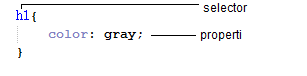
\includegraphics[scale=0.8]{Gambar/selector-ex}
			\caption{Format Penulisan Definisi CSS} 
			\label{fig:2_selector_ex}
		\end{figure}
Beberapa jenis CSS \textit{Selector} antara lain:
\begin{enumerate}
	\item \textit{\textbf{Element selector}}, memilih \textit{tag} HTML.\\
		Contoh: \texttt{h1}\\
		Keterangan: \textit{selector} mendefinisikan elemen h1.
	\item \textit{\textbf{Grouping Selector}}, memilih beberapa \textit{selector} sekaligus. Setiap \textit{selector} dipisahkan dengan ``,''.\\
		Contoh: \texttt{h1, h2, p}\\
		Keterangan: \textit{selector} mendefinisikan elemen h1, h2, dan p.
	\item \textit{\textbf{Universal Selector}}, memilih seluruh elemen. \textit{Selector} ditampilkan sebagai ``*''.\\
		Contoh: \texttt{*}\\
		Keterangan: \textit{selector} mendefinisikan seluruh elemen.
	\item \textit{\textbf{Class Selector}}, memilih kelas elemen. \textit{Selector} ditampilkan sebagai ``.'' kemudian diikuti nama kelas elemen.\\
		Contoh: \texttt{.top}\\
		Keterangan: \textit{selector} mendefinisikan elemen dengan kelas ``top''.
	\item \textit{\textbf{ID Selector}}, memilih ID elemen. \textit{Selector} ditampilkan sebagai ``\#'' kemudian diikuti ID elemen.\\
		Contoh: \texttt{\#top}\\
		Keterangan: \textit{selector} mendefinisikan elemen dengan ID ``top''. 
	\item \textit{\textbf{Attribute Selector}}, akan dijelaskan dua \textit{attribute selector} yaitu:
		\begin{itemize}
			\item \textit{\textbf{Simple Attribute}}, memilih atribut elemen. \textit{Selector} ditampilkan sebagai nama atribut kemudian diapit dengan kurung siku.
			Contoh: \texttt{[name]}\\
			Keterangan: \textit{selector} mendefinisikan elemen dengan atribut ``name''. 
			
			\item \textit{\textbf{Exact Value Attribute}}, memilih atribut elemen dengan nilai tertentu. \textit{Selector} ditampilkan sebagai definisi atribut kemudian diapit dengan kurung siku.
			Contoh: \texttt{[name=Joe]}\\
			Keterangan: \textit{selector} mendefinisikan elemen dengan atribut ``name'' yang memiliki nilai ``Joe''. 
		\end{itemize}
		
	\item \textit{\textbf{Descendant Selector}}, memilih \textit{child} elemen yang merupakan keturunan \textit{parent} tertentu. \textit{Selector} ditampilkan dengan mendefinisikan parent kemudian diikuti oleh child dipisahkan dengan spasi.\\
			Contoh: \texttt{p .top}\\
			Keterangan: \textit{selector} mendefinisikan elemen dengan kelas ``top'' yang merupakan \textit{child} dari elemen p. 
\end{enumerate}		

\section{Chrome DevTools}
\label{sec:devtools}

Chrome Developer Tools (DevTools) adalah perangkat \textit{debugging} yang dimiliki Google Chrome\cite{devtools}. Saat menunjungi suatu halaman web, pengguna DevTools dapat melakukan \textit{debugging} pada halaman tersebut. DevTools dapat diakses dengan menekan ``Ctrl+Shift+I'' saat sedang membuka suatu halaman web.  

Panel-panel yang dimiliki DevTools (Gambar \ref{fig:2_chrome_devtools}) antara lain:
\begin{enumerate}
	\item \textbf{Elements}, memeriksa dan mengubah elemen HTML dan \textit{style} dari suatu situs web.
	\item \textbf{Console}, mendapatkan informasi pengembangan dan berinteraksi dengan dokumen.
	\item \textbf{Sources}, melakukan \textit{debugging} pada JavaScript dengan menentukan \textit{breakpoint}.
	\item \textbf{Network}, memantau aktivitas jaringan pada situs web secara \textit{real-time}.
	\item \textbf{Audits}, menganalisis halaman yang dimuat.
	\item \textbf{Timeline}, menampilkan alur waktu saat memuat halaman.
	\item \textbf{Profiles}, menggambarkan waktu eksekusi dan penggunaan memori saat memuat halaman.
	\item \textbf{Resources}, memeriksa sumber daya halaman yang dapat berupa basis data, \textit{cookies}, dan \textit{cache}.
\end{enumerate}

\begin{figure}[H]
	\centering
	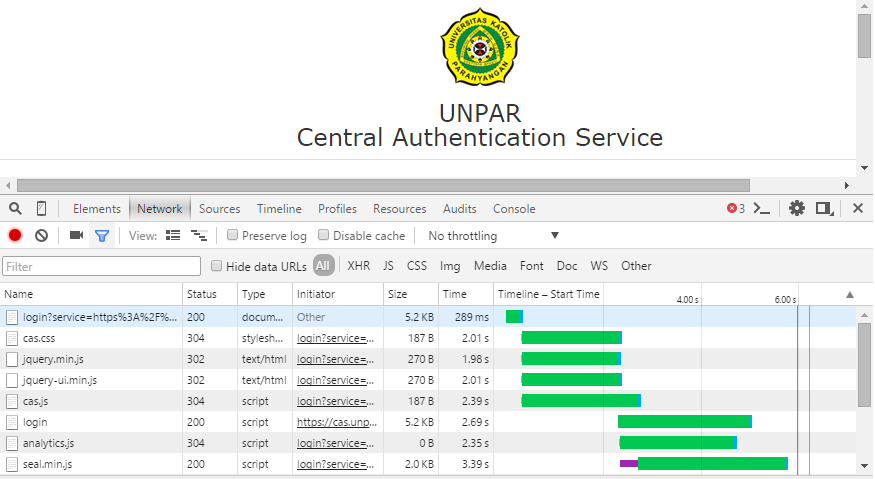
\includegraphics[scale=0.5]{Gambar/chrome-devtools}
	\caption{Chrome DevTools} 
	\label{fig:2_chrome_devtools}
\end{figure}

Pada subbab-subbab berikut akan dijelaskan mengenai dua panel dari DevTools.

\subsection{Elements}
Panel Elements memungkinkan untuk memperlihatkan informasi yang terstruktur tentang halaman yang sedang dibuka. HTML akan ditampilkan dalam bentuk pohon \textit{Document Object Model} (DOM). DOM adalah sebuah struktur seperti pohon yang dibuat oleh browser untuk menemukan elemen HTML\footnote{\url{http://try.jquery.com/}, diakses 24 September 2015}. Tampilan pohon DOM memperlihatkan struktur DOM dari halaman yang sedang dibuka. Pohon DOM adalah pohon dari node-node yang mewakili setiap elemen HTML seperti \texttt{<body>} dan \texttt{<p>}. 

Pemeriksaan elemen akan memperlihatkan node DOM dan CSS dari elemen yang dipilih pada \textit{browser}. Pemeriksaan elemen dapat dilakukan dengan cara klik kanan pada elemen yang ingin diperiksa kemudian pilih ``Inspect element''. Dengan melakukan pemeriksaan elemen, jendela panel Elements akan muncul. Sebagai contoh pada Gambar \ref{fig:2_elements_panel}, saat melakukan ``Inspect element'' pada nama mahasiswa, panel Elements akan muncul dan menunjukkan pohon DOM dari halaman tersebut. Selain itu panel Elements juga menunjukkan CSS selector dari elemen tersebut yaitu \texttt{p.student-name}.

\begin{figure}[H]
	\centering
	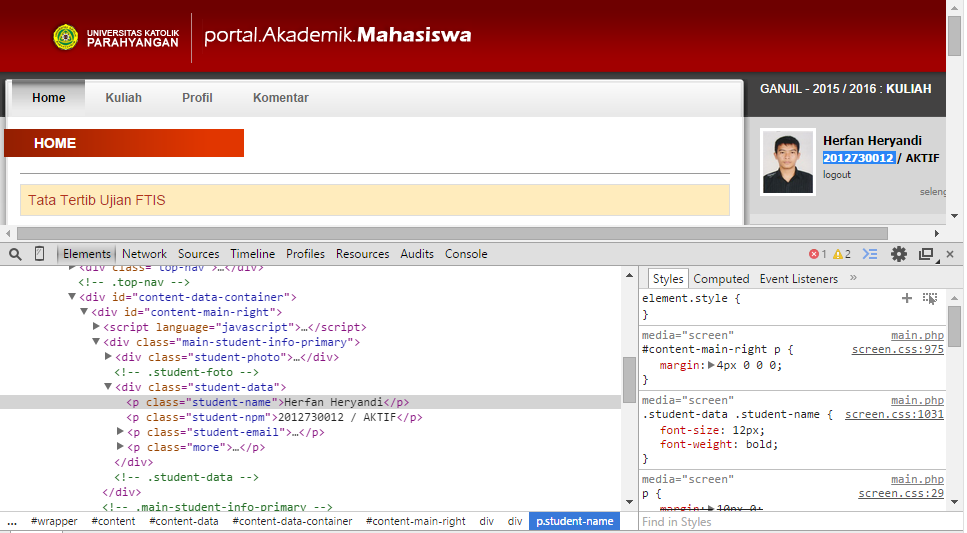
\includegraphics[scale=0.5]{Gambar/elements-panel}
	\caption{Panel Elements} 
	\label{fig:2_elements_panel}
\end{figure}

\subsection{Network}
Panel Network secara otomatis merekam semua aktivitas jaringan saat DevTools terbuka. Pertama kali dibuka, panel Network masih kosong. Halaman web harus dimuat ulang untuk mulai merekam aktivitas jaringan atau menunggu adanya aktivitas jaringan pada halaman web. Panel Network akan mencatat sumber daya dari aktivitas jaringan yang terekam. Setiap sumber daya akan ditambahkan ke dalam sebuah baris dalam tabel Network seperti pada Gambar \ref{fig:2_network_panel} dengan rincian kolom sebagai berikut:
\begin{itemize}
	\item \textbf{Name dan Path}, nama dan URL dari sumber daya.
	\item \textbf{Method}, metode permintaan HTTP.
	\item \textbf{Status dan Text}, kode status HTTP dan pesan.
	\item \textbf{Domain}, domain dari sumber daya.
	\item \textbf{Type}, tipe sumber daya yang diminta.
	\item \textbf{Cookies}, banyaknya \textit{cookie} yang dikirim dalam permintaan.
	\item \textbf{Size dan Content}, \textit{size} merupakan ukuran dari \textit{header} dan \textit{body} jawaban yang dikirim server sedangkan \textit{content} merupakan ukuran konten sumber daya.
	\item \textbf{Timeline}, alur waktu dari seluruh aktivitas jaringan yang diminta.
\end{itemize}

\begin{figure}[H]
	\centering
	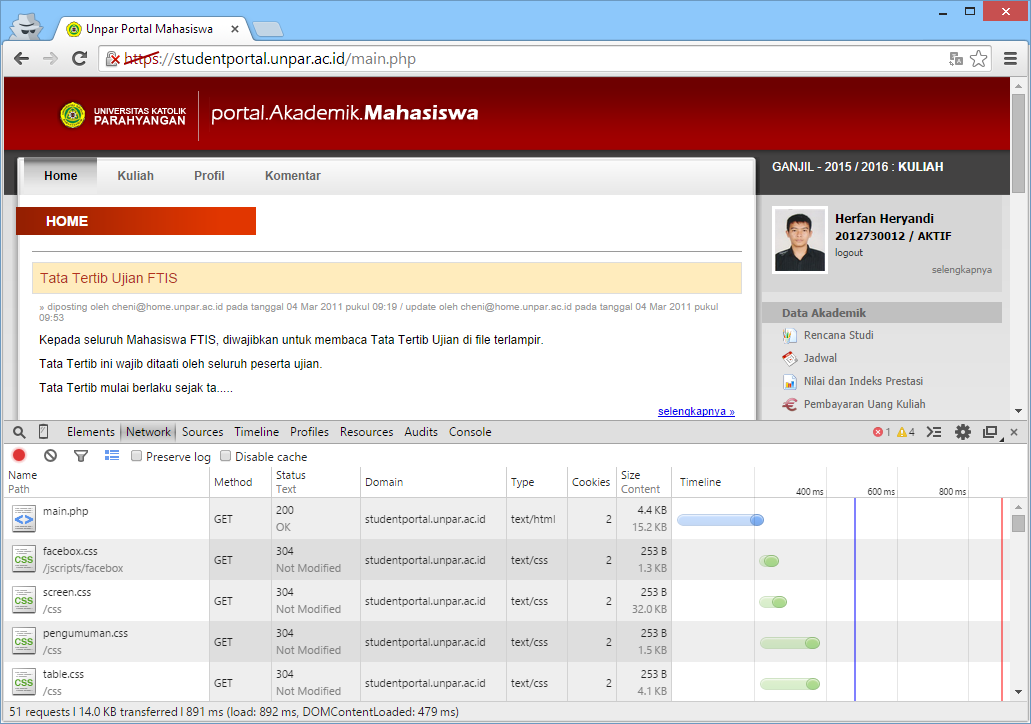
\includegraphics[scale=0.5]{Gambar/network-panel}
	\caption{Panel Network} 
	\label{fig:2_network_panel}
\end{figure}


Ketika nama sumber daya dalam tabel Network diklik, maka akan muncul tautan baru yang berisi rincian tambahan sebagai berikut:
\begin{itemize}
	\item \textbf{Header}\\
	Tautan Header menampilkan \textit{request} URL, \textit{request method}, \textit{status code}, HTTP \textit{response} dan \textit{request header} beserta nilainya, dan \textit{query string parameter}. HTTP header dapat ditampilkan secara terformat atau dalam bentuk sumber dengan mengklik tombol \textit{toggle} ``view parsed''/``view source''. Nilai-nilai parameter dapat ditampilkan dalam bentuk yang sudah didekodekan atau dalam bentuk URL yang dienkode dengan mengklik tombol \textit{toggle} ``view decoded''/``view URL encoded''. Sebagai contoh, Gambar \ref{fig:2_network_get} menampilkan \textit{header} pada metode permintaan GET sedangkan Gambar \ref{fig:2_network_post} menampilkan \textit{header} pada metode permintaan POST.
	
\begin{figure}[H]
	\centering
	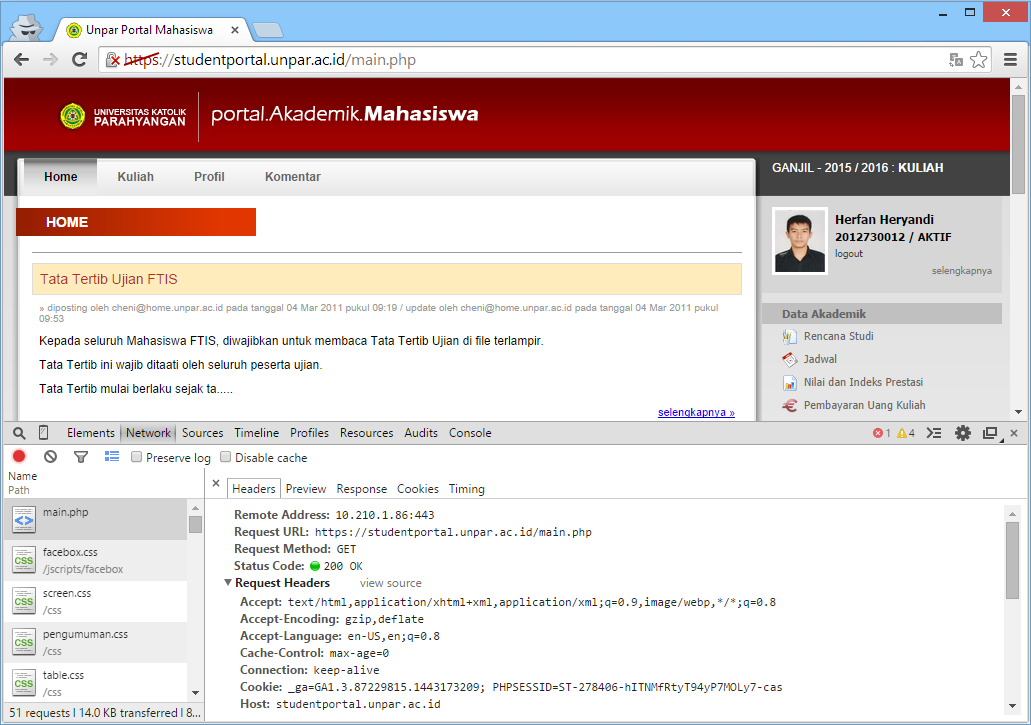
\includegraphics[scale=0.5]{Gambar/network-header}
	\caption{Contoh Tautan Header pada Metode Permintaan GET} 
	\label{fig:2_network_get}
\end{figure}

\begin{figure}[H]
	\centering
	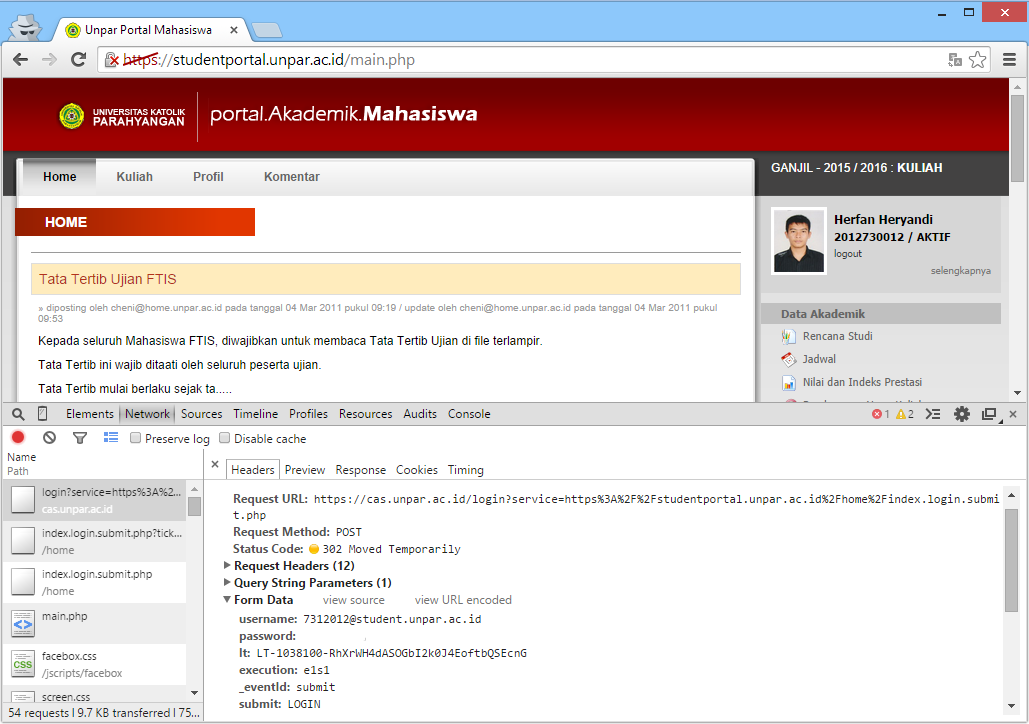
\includegraphics[scale=0.5]{Gambar/network-post}
	\caption{Contoh Tautan Header pada Metode Permintaan POST} 
	\label{fig:2_network_post}
\end{figure}

	\item \textbf{Preview}\\
	Tautan Preview menampilkan \textit{preview} sumber daya jika tersedia. Gambar \ref{fig:2_network_prev_available} menampilkan \textit{preview} yang tersedia pada sumber daya. Jika \textit{preview} tidak tersedia maka akan tampilan akan sama dengan jawaban seperti yang terlihat pada Gambar \ref{fig:2_network_prev_notavailable}.
	
\begin{figure}[H]
	\centering
	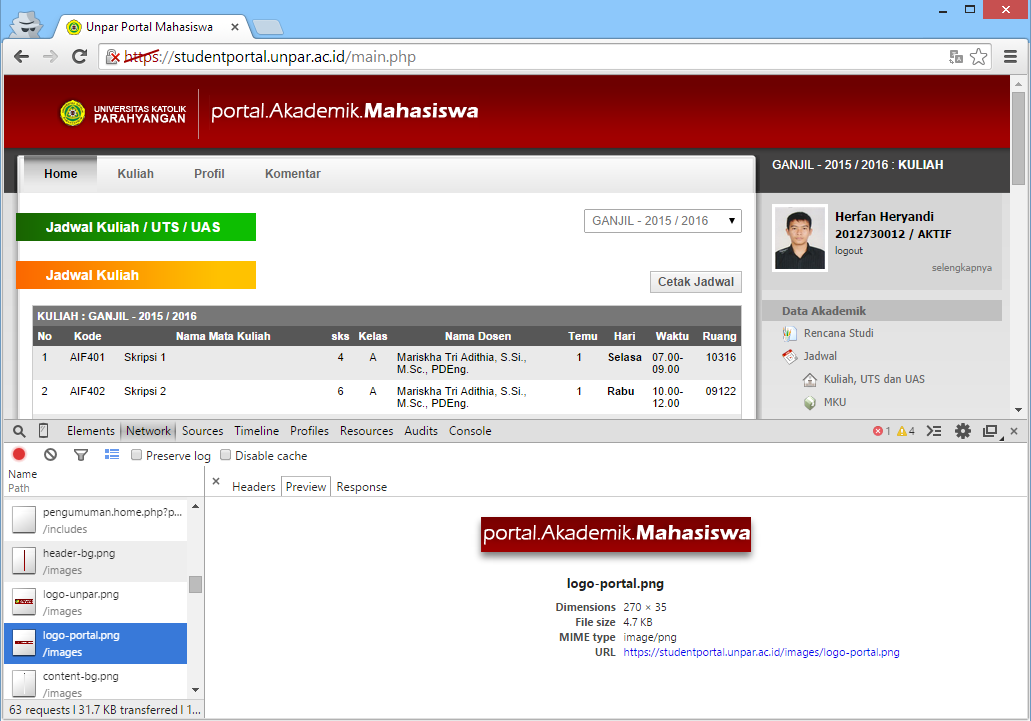
\includegraphics[scale=0.5]{Gambar/network-preview-available}
	\caption{Contoh \textit{Preview} yang Tersedia} 
	\label{fig:2_network_prev_available}
\end{figure}

\begin{figure}[H]
	\centering
	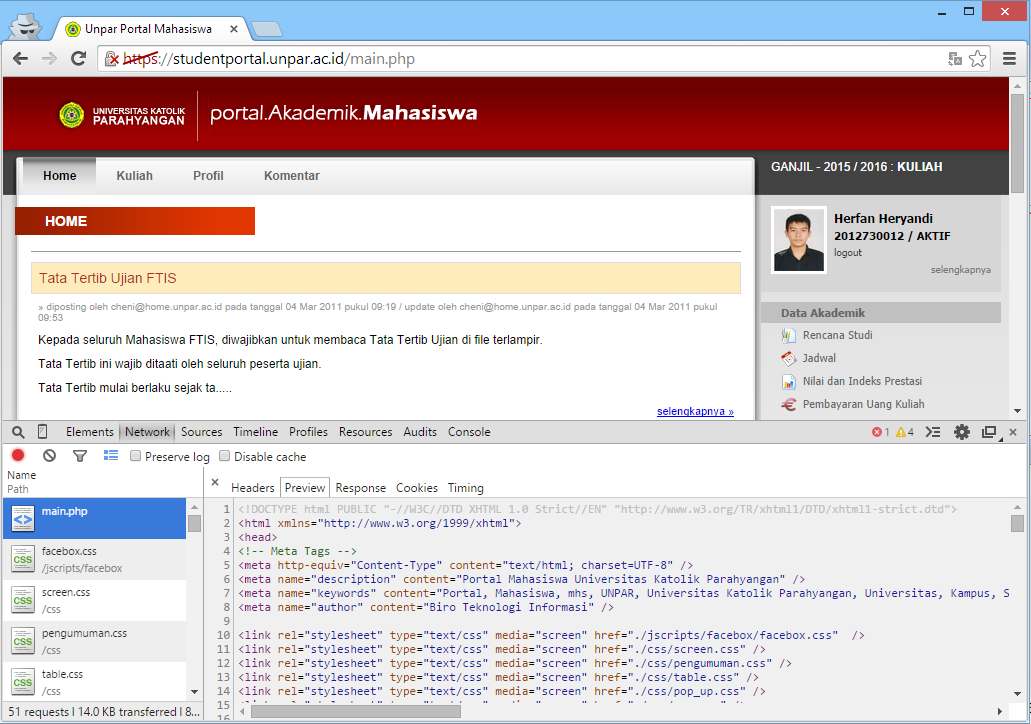
\includegraphics[scale=0.5]{Gambar/network-preview-notAvailable}
	\caption{Contoh \textit{Preview} yang Tidak Tersedia} 
	\label{fig:2_network_prev_notavailable}
\end{figure}

	\item \textbf{Response}\\
	Tautan Response berisi konten sumber daya yang tidak terformat. Sebagai contoh pada Gambar \ref{fig:2_network_response} menampilkan tautan Response dari sumber daya \texttt{main.php}.
\begin{figure}[H]
	\centering
	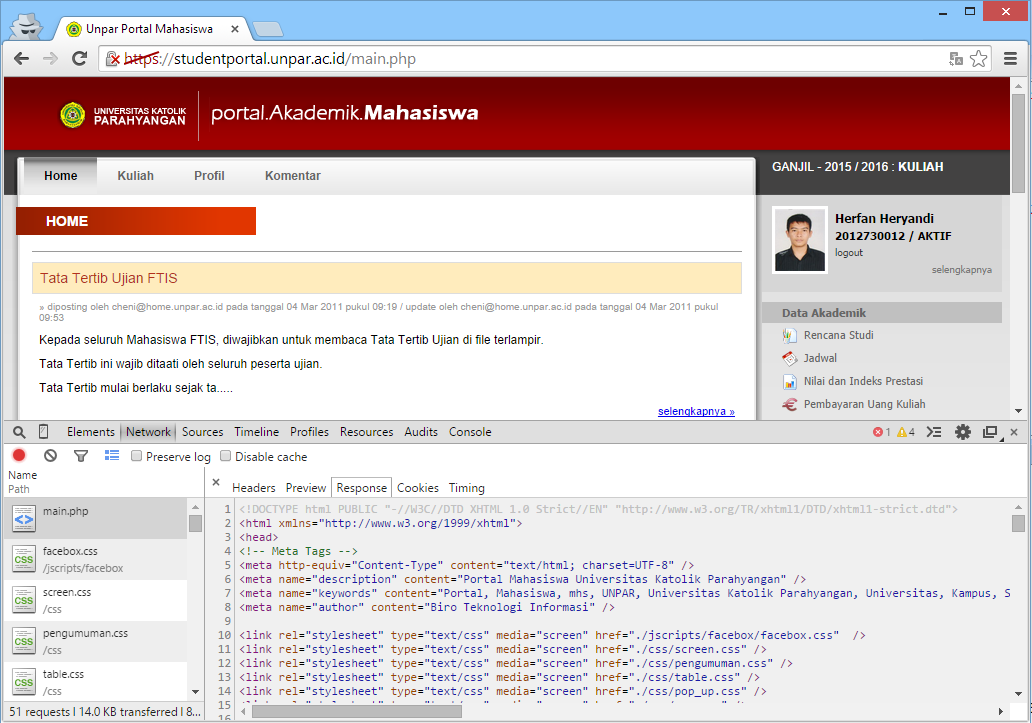
\includegraphics[scale=0.5]{Gambar/network-response}
	\caption{Contoh Tautan Response} 
	\label{fig:2_network_response}
\end{figure}

	\item \textbf{Cookies}\\
	Tautan Cookies menampilkan sebuah tabel yang terdiri dari seluruh \textit{cookie} yang ditransmisikan dalam \textit{header} permintaan dan jawaban HTTP. Contoh dari tabel \textit{cookie} dapat dilihat pada Gambar \ref{fig:2_network_cookies} dengan rincian kolom sebagai berikut:
	\begin{itemize}
		\item \textbf{Name}, nama \textit{cookie}
		\item \textbf{Value}, nilai \textit{cookie}
		\item \textbf{Domain}, domain yang memiliki \textit{cookie}
		\item \textbf{Path}, URL asal \textit{cookie}
		\item \textbf{Expires/Max-Age}, batas akhir nilai \textit{cookie}
		\item \textbf{Size}, ukuran \textit{cookie} dalam byte
		\item \textbf{HTTP}, menunjukkan bahwa \textit{cookie} harus ditetapkan oleh browser dalam permintaan HTTP, dan tidak dapat diakses dengan JavaScript
		\item \textbf{Secure}, menunjukkan bahwa \textit{cookie} harus dikirim melalui koneksi yang aman
	\end{itemize}
	
\begin{figure}[H]
	\centering
	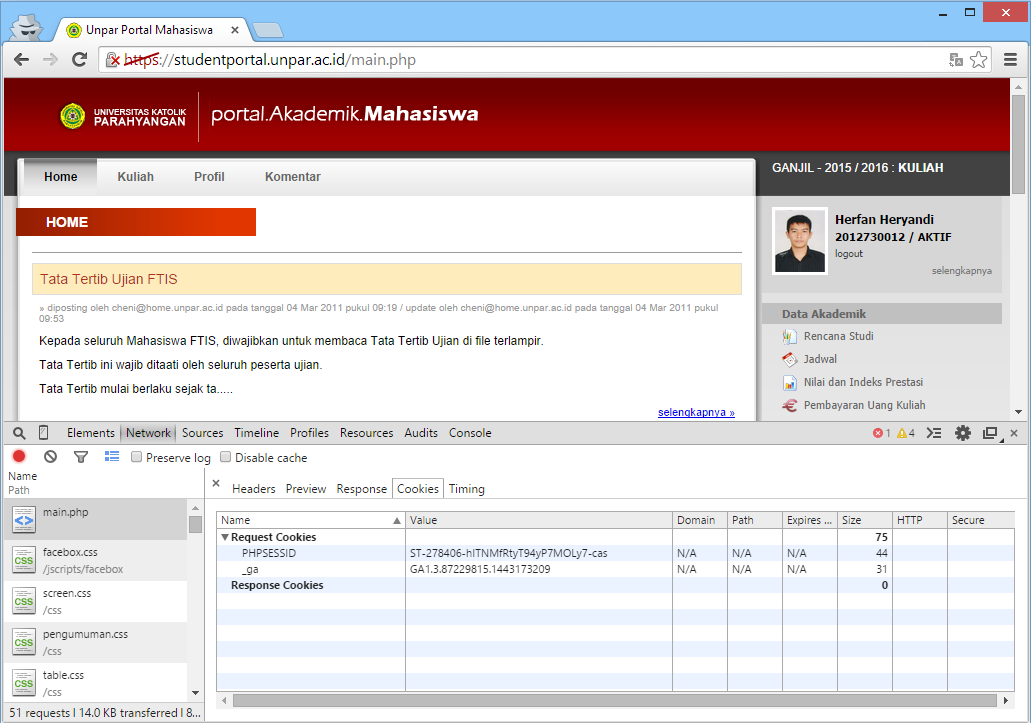
\includegraphics[scale=0.5]{Gambar/network-cookies}
	\caption{Contoh Tabel pada Tautan Cookie} 
	\label{fig:2_network_cookies}
\end{figure}

\end{itemize}

\section{Play Framework}
\label{sec:play}

Play Framework\cite{Leroux:2014} merupakan sebuah web \textit{framework} berbasis bahasa Java dan Scala. Play Framework juga menggunakan arsitektur \textit{Model-View-Controller} (MVC) di mana \textit{model} dan \textit{controller} menggunakan bahasa Java sedangkan \textit{view} menggunakan bahasa Scala dan HTML. Agar dapat berjalan, Play Framework membutuhkan sistem operasi dan Java Development Kit (JDK). Struktur aplikasi Play Framework dapat dilihat pada Gambar \ref{fig:2_play_dir}.
\begin{figure}[H]
	\centering
	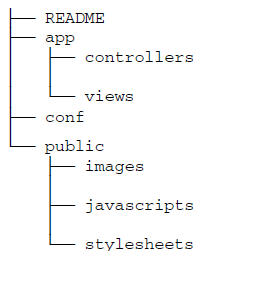
\includegraphics[scale=0.5]{Gambar/play-dir}
	\caption{Struktur Aplikasi Play Framework} 
	\label{fig:2_play_dir}
\end{figure}

Dalam direktori \texttt{conf}, terdapat file \texttt{routes}. Melalui \texttt{routes}, rute aplikasi dapat ditentukan dengan memetakan URL ke kode aplikasi. Setiap \texttt{route} memiliki tiga bagian yaitu HTTP \textit{method}, URL \textit{path}, dan \textit{action method}.  HTTP \textit{method} merupakan metode pengiriman HTTP. URL \textit{path} merupakan URL untuk mengakses halaman. \textit{Action method} merupakan \textit{method} yang menangani permintaan metode pengiriman HTTP. Sebagai contoh pada Gambar \ref{fig:2_routes_example}, setiap permintaan GET pada URL \texttt{/list} akan ditangani oleh \textit{method} \texttt{list}() milik kelas \texttt{Products} yang terdapat pada \textit{package} \texttt{controllers}.

\begin{figure}[H]
	\centering
	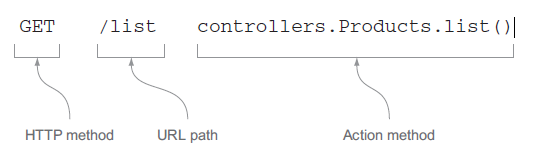
\includegraphics[scale=0.5]{Gambar/contoh-routes}
	\caption{Contoh Komponen \texttt{Route}\cite{Leroux:2014}} 
	\label{fig:2_routes_example}
\end{figure}

Direktori \texttt{app} merupakan sumber dari kode program seperti file Java dan \textit{view}. Saat pertama kali proyek Play Framework dibuat, direktori \texttt{app} berisi file-file seperti pada Gambar \ref{fig:2_app_dir}. Dalam folder \texttt{controllers}, terdapat file \texttt{Application.java} yang berisi kode Java untuk menghasilkan halaman web. Kelas yang menangani permintaan HTTP dan mengembalikan hasil HTTP disebut kelas \textit{controller}. Kelas \textit{controller} merupakan kelas yang memiliki \textit{action method}. Setiap \textit{action method} memiliki tipe kembalian \textit{Result} yang merepresentasikan \textit{view}. Pada buku referensi\cite{Leroux:2014}, tertulis bahwa kembalian dari \textit{action method} harus \texttt{static} tetapi pada versi Play Framework 2.4, \texttt{static} dihilangkan. \textit{Action method} akan berhubungan dengan \textit{view} setelah didefinisikan di \texttt{routes}. \textit{Controller} dapat mengirimkan parameter pada \textit{view} melalui kembalian dari \textit{action method}. Berikut ini adalah contoh \textit{method} pada kelas \textit{Controller}:
\begin{lstlisting}
public Result home(){
	String nama = mahasiswa.getNama();
	return ok(views.html.home.render(nama));
}
\end{lstlisting}
\textit{Method} \texttt{home()} mengembalikan \textit{view} \texttt{home} yang berada pada \textit{package} \texttt{views} dengan mengirim \textit{parameter} ``nama''.

\begin{figure}[H]
	\centering
	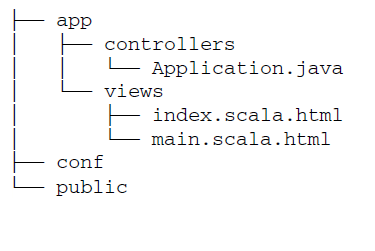
\includegraphics[scale=0.5]{Gambar/app-dir}
	\caption{Direktori \texttt{app} yang Dibangkitkan Play Framework\cite{Leroux:2014}} 
	\label{fig:2_app_dir}
\end{figure}

Dalam folder \texttt{views} terdapat dua file yaitu \texttt{index.scala.html} dan \texttt{main.scala.html} yang berfungsi untuk mendefinisikan halaman HTML. Setiap konten yang dihasilkan pada server dan dikirim ke klien dalam \textit{body} HTTP, seperti halaman HTML, disebut \textit{view}. \textit{View} dapat menerima parameter dari \textit{controller} menggunakan bahasa Scala. Berikut contoh penggunaan bahasa Scala pada \textit{view} dalam penerimaan parameter:
\begin{lstlisting}
@(message: String)

<!DOCTYPE HTML>

<html lang=``en''>
	<head>
		<title>Informatika Student Portal</title>
	</head>
	<body>
		Nama: @message
	</body>
<html>
\end{lstlisting}
Pada baris pertama ``message'' mendefinisikan nama parameter yang diterima dengan tipe \textit{String}. Tipe yang diterima \textit{view} harus sama dengan tipe yang dikirim \textit{controller} begitu pula banyak parameternya. Baris ke-10 menampilkan ``message'' pada halaman HTML. Tanda ``@'' menandakan penggunaan bahasa Scala pada \textit{view}. Bahasa Scala pada Play Framework merupakan \textit{scala template} yaitu \textit{template} dengan \textit{syntax} berbasis bahasa Scala sehingga penulisan bahasa Scala pada Play Framework berbeda dengan penulisan bahasa Scala pada umumnya.

Direktori \texttt{public} berisi sumber yang dapat diakses secara langsung sebagai aset publik. Biasanya aset publik mendukung file selain aplikasi yang dibuat seperti gambar, \textit{stylesheet}, Javascript, dan halaman HTML statis. Aset publik tidak dihasilkan oleh aplikasi melainkan diatur secara langsung oleh pembuat program.

Dalam Play Framework, objek yang disimpan pada \textit{session} memiliki masa hidup yaitu selama \textit{browser} dibuka. \textit{Session} tidak disimpan di server melainkan ditambahkan ke setiap permintaan HTTP berikutnya menggunakan mekanisme \textit{cookie}. Ukuran data \textit{session} sangat terbatas yaitu hingga 4 KB sehingga hanya dapat menyimpan \textit{String}. Pada controller, \textit{session} dapat disimpan dengan \textit{method}:
	\begin{itemize}
			\item \textbf{public static void session(String key, String value)} \\
				\textbf{Parameter:}
				\begin{itemize}
					\item \textbf{key} kunci \textit{session}.
					\item \textbf{value} nilai \textit{session}.
				\end{itemize}
	\end{itemize}
 Sedangkan nilai \textit{session} dapat diperoleh menggunakan \textit{method}: 
\begin{itemize}
			\item \textbf{public static String session(String key)} \\
				\textbf{Parameter:}
				\begin{itemize}
					\item \textbf{key} kunci \textit{session}.
				\end{itemize}
				\textbf{Kembalian:} nilai \textit{session}.
	\end{itemize}


\section{SIA Models}
\label{sec:siamodels}
SIA Models merupakan kelas-kelas dalam bahasa Java yang merepresentasikan Sistem Informasi Akademik Teknik Informatika UNPAR\cite{siamodels}. Berdasarkan diagram kelas SIA Models (Gambar \ref{fig:2_siamodels_class}), kelas-kelas yang dimiliki SIA Models terbagi ke dalam tiga \textit{package} antara lain:

\begin{figure}[H]
	\centering
	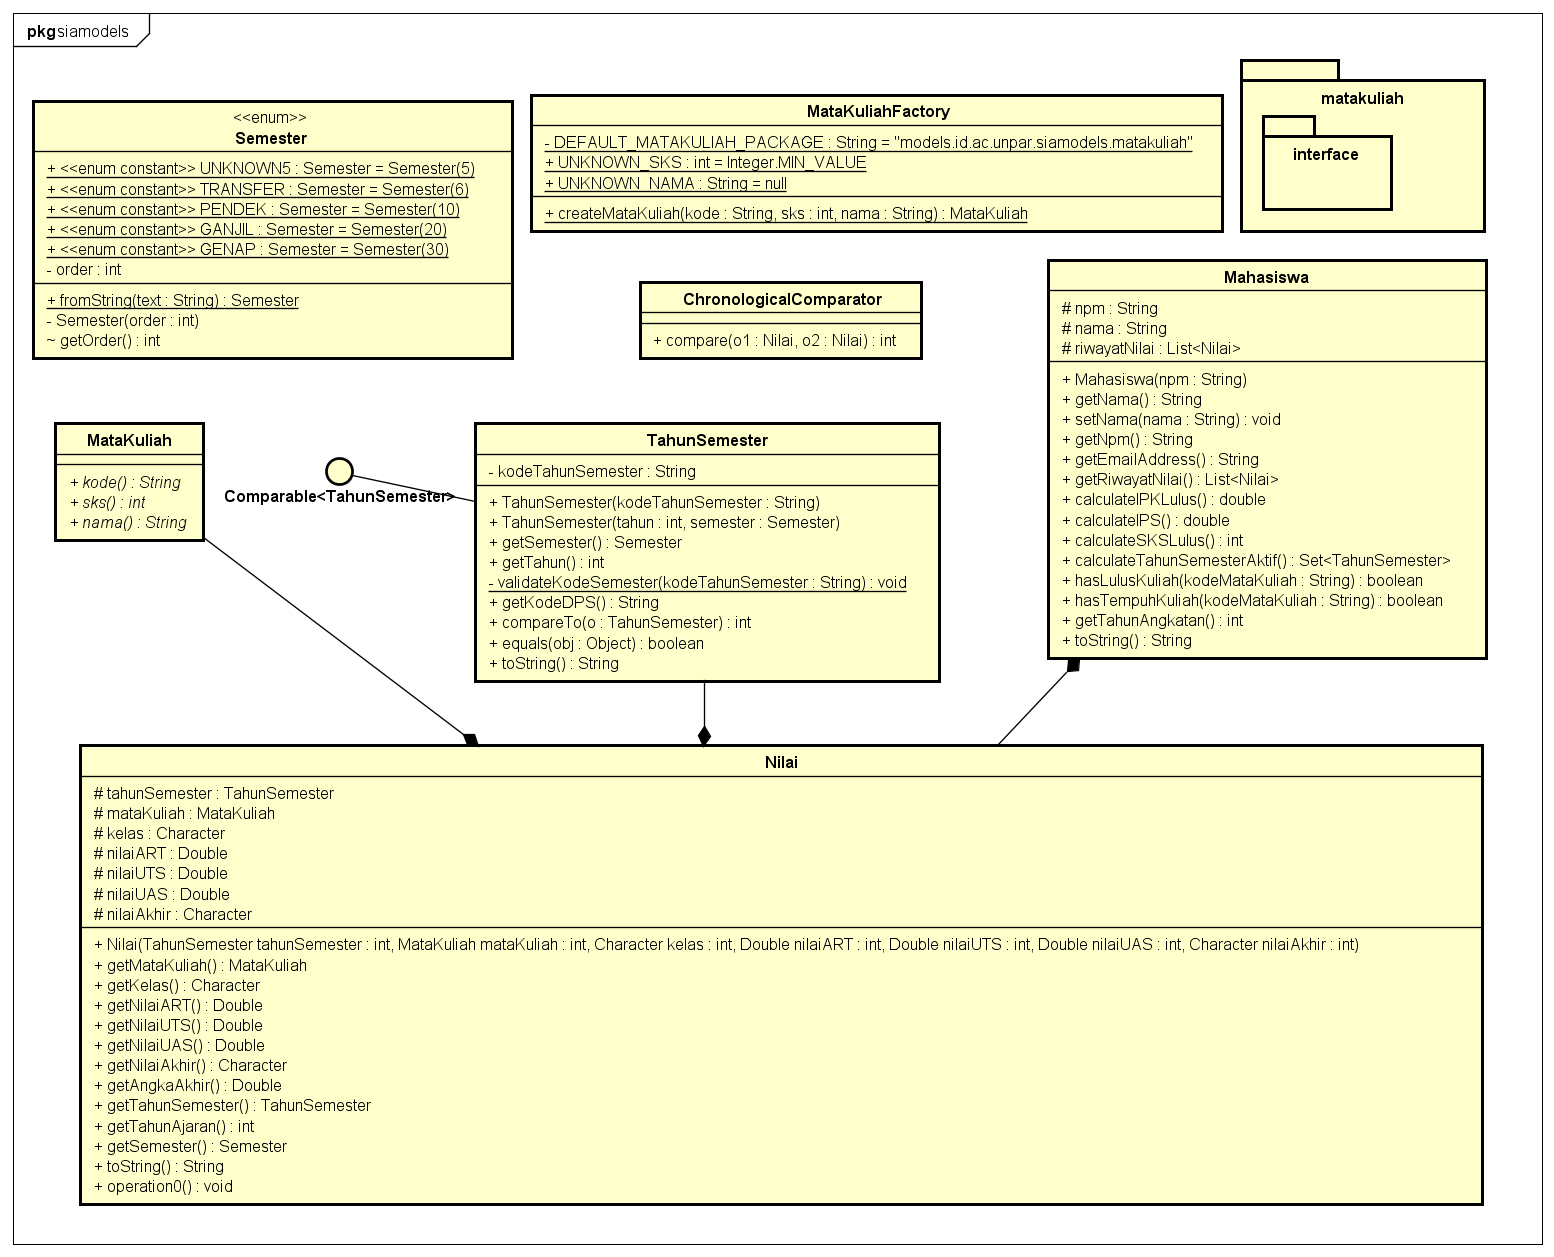
\includegraphics[scale=0.35]{Gambar/siamodels-class}
	\caption{Diagram Kelas SIA Models} 
	\label{fig:2_siamodels_class}
\end{figure}

\begin{enumerate}
	\item \textit{Package} \texttt{id.ac.unpar.siamodels}\\
	\textit{Package} ini memiliki kelas-kelas sebagai berikut:
	\begin{enumerate}
		\item Mahasiswa\\
		Kelas ini merepresentasikan mahasiswa. Atribut yang dimiliki kelas ini antara lain:
		\begin{itemize}
			\item \textbf{String npm:} Nomor Pokok Mahasiswa (NPM).
			\item \textbf{String nama:} nama mahasiswa.
			\item \textbf{List<Nilai> riwayatNilai:} riwayat nilai yang dimiliki mahasiswa.
		\end{itemize}
	\textit{Method-method} yang dimiliki kelas ini adalah sebagai berikut:
		\begin{itemize}
			\item \textbf{public Mahasiswa(String npm)}\\
			Merupakan \textit{constructor} dari kelas Mahasiswa.\\
			\textbf{Parameter:}
			\begin{itemize}
				\item \textbf{npm} nomor pokok mahasiswa.
			\end{itemize}
			
			\item \textbf{public String getNama()}\\
				Berfungsi untuk mendapatkan nama mahasiswa.\\
				\textbf{Kembalian:} nama mahasiswa.

			\item \textbf{public void setNama(String nama)}\\
				Berfungsi untuk mengubah nama mahasiswa.\\
				\textbf{Parameter:}
				\begin{itemize}
					\item \textbf{nama} nama mahasiswa.
				\end{itemize}
		
			\item \textbf{public String getNpm()}\\
				Berfungsi untuk mendapatkan nomor pokok mahasiswa.\\
				\textbf{Kembalian:} nomor pokok mahasiswa.
			
			\item \textbf{public String getEmailAddress()}\\
				Berfungsi untuk mendapatkan \textit{email} mahasiswa.\\
				\textbf{Kembalian:} \textit{email} mahasiswa.
			
			\item \textbf{public List<Nilai> getRiwayatNilai()}\\
				Berfungsi untuk mendapatkan riwayat nilai mahasiswa.\\
				\textbf{Kembalian:} riwayat nilai mahasiswa dalam List.
				
			\item \textbf{public double calculateIPKLulus()}\\
				Menghitung IPK mahasiswa sampai saat ini, dengan aturan kuliah yang tidak lulus tidak dihitung dan jika pengambilan beberapa kali, diambil nilai terbaik. Sebelum memanggil \textit{method} ini, \texttt{getRiwayatNilai()} harus sudah mengandung nilai per mata kuliah.\\
				\textbf{Kembalian:} IPK lulus.
				
			\item \textbf{public double calculateIPS()}\\
				Menghitung IPS semester terakhir sampai saat ini, dengan aturan kuliah yang tidak lulus dihitung. Sebelum memanggil \textit{method} ini, \texttt{getRiwayatNilai()} harus sudah mengandung nilai per mata kuliah.\\
				\textbf{Kembalian:}  nilai IPS sampai saat ini.
				
			\item \textbf{public int calculateSKSLulus()}\\
				Menghitung jumlah SKS lulus mahasiswa saat ini. Sebelum memanggil \textit{method} ini, \texttt{getRiwayatNilai()} harus sudah mengandung nilai per mata kuliah.\\
				\textbf{Kembalian:} SKS lulus.
				
			\item \textbf{public Set<TahunSemester> calculateTahunSemesterAktif()}\\
				Mendapatkan seluruh tahun semester di mana mahasiswa ini tercatat sebagai mahasiswa aktif, dengan strategi memeriksa riwayat nilainya.Jika ada satu nilai saja pada sebuah tahun semester, maka dianggap aktif pada semester tersebut.\\
				\textbf{Kembalian:} kumpulan tahun semester di mana mahasiswa ini aktif.
				
			\item \textbf{public boolean hasLulusKuliah(String kodeMataKuliah)}\\
				Memeriksa apakah mahasiswa ini sudah lulus mata kuliah tertentu. Sebelum memanggil \textit{method} ini, \texttt{getRiwayatNilai()} harus sudah mengandung nilai per mata kuliah.\\
				\textbf{Parameter:}
				\begin{itemize}
					\item \textbf{kodeMataKuliah} kode mata kuliah yang ingin diperiksa kelulusannya.
				\end{itemize}
				\textbf{Kembalian:} \texttt{true} jika sudah pernah mengambil dan lulus, \texttt{false} jika belum.
				
			\item \textbf{public boolean hasTempuhKuliah(String kodeMataKuliah)}\\
				Memeriksa apakah mahasiswa ini sudah pernah menempuh mata kuliah tertentu. Sebelum memanggil \textit{method} ini, \texttt{getRiwayatNilai()} harus sudah mengandung nilai per mata kuliah.\\
				\textbf{Parameter:}
				\begin{itemize}
					\item \textbf{kodeMataKuliah} kode mata kuliah yang ingin diperiksa kelulusannya.
				\end{itemize}
				\textbf{Kembalian:} \texttt{true} jika sudah pernah mengambil, \texttt{false} jika belum.
			
			\item \textbf{public int getTahunAngkatan()}\\
				Mendapatkan tahun angkatan mahasiswa ini berdasarkan NPM-nya.\\
				\textbf{Kembalian:} tahun angkatan.
			\end{itemize}
		
		\item Nilai\\
		Kelas ini merepresentasikan nilai yang ada pada riwayat nilai mahasiswa. Atribut yang dimiliki kelas ini antara lain:
		\begin{itemize}
			\item \textbf{TahunSemester tahunSemester:} tahun dan semester kuliah ini diambil
			\item \textbf{MataKuliah mataKuliah:} mata kuliah yang diambil.
			\item \textbf{Character kelas:} kelas kuliah.
			\item \textbf{Double nilaiART:} nilai Angka Rata-rata Tugas (ART).
			\item \textbf{Double nilaiUTS:} nilai Ujian Tengah Semester (UTS).
			\item \textbf{Double nilaiUAS:} nilai Ujian Akhir Semester (UAS).
			\item \textbf{Character nilaiAkhir:} nilai akhir.
		\end{itemize}
	\textit{Method-method} yang dimiliki kelas ini adalah sebagai berikut:
		\begin{itemize}
			\item \textbf{public Nilai(TahunSemester tahunSemester, MataKuliah mataKuliah, Character kelas, Double nilaiART, Double nilaiUTS, Double nilaiUAS, Character nilaiAkhir)}\\
				Merupakan \textit{constructor} dari kelas Nilai.\\
				\textbf{Parameter:}
				\begin{itemize}
					\item \textbf{tahunSemester} tahun dan semester kuliah ini diambil.
					\item \textbf{mataKuliah} mata kuliah yang diambil.
					\item \textbf{kelas} kelas kuliah.
					\item \textbf{nilaiART} nilai ART.
					\item \textbf{nilaiUTS} nilai UTS.
					\item \textbf{nilaiUAS} nilai UAS.
					\item \textbf{nilaiAkhir} nilai akhir.
				\end{itemize}
				
			\item \textbf{public MataKuliah getMataKuliah()}\\
				Mendapatkan mata kuliah yang diambil.\\
				\textbf{Kembalian:} mata kuliah.
				
			\item \textbf{public Character getKelas()}\\
				Mendapatkan kelas kuliah.\\
				\textbf{Kembalian:} kelas kuliah.
				
			\item \textbf{public Double getNilaiART()}\\
				Mendapatkan nilai ART.\\
				\textbf{Kembalian:} nilai ART.
				
			\item \textbf{public Double getNilaiUTS()}\\
				Mendapatkan nilai UTS.\\
				\textbf{Kembalian:} nilai UTS.
				
			\item \textbf{public Double getNilaiUAS()}\\
				Mendapatkan nilai UAS.\\
				\textbf{Kembalian:} nilai UAS.
				
			\item \textbf{public Double getNilaikhir()}\\
				Mendapatkan nilai akhir dalam bentuk angka.\\
				\textbf{Kembalian:} nilai akhir dalam huruf atau \texttt{null} jika tidak ada.
			
			\item \textbf{public Double getAngkaAkhir()}\\
				Mengembalikan nilai akhir dalam bentuk huruf (A, B, C, D, ...).\\
				\textbf{Kembalian:} nilai akhir dalam angka, atau \texttt{null} jika \texttt{getNilaiAkhir()} mengembalikan \texttt{null}.
			
			\item \textbf{public int getTahunAjaran()}\\
				Mendapatkan tahun ajaran saat pengambilan mata kuliah.\\
				\textbf{Kembalian:} tahun ajaran saat pengambilan mata kuliah.
			
			\item \textbf{public TahunSemester getTahunSemester()}\\
				Mendapatkan tahun dan semester pengambilan mata kuliah.\\
				\textbf{Kembalian:} tahun dan semester pengambilan mata kuliah.	
				
			\item \textbf{public Semester getSemester()}\\
				Mendapatkan semester pengambilan mata kuliah.\\
				\textbf{Kembalian:} semester pengambilan mata kuliah
		\end{itemize}
		
		\item ChronologicalComparator\\
		Pembanding antara satu nilai dengan nilai lainnya, secara kronologis waktu pengambilan. \textit{Method} yang dimiliki kelas ini adalah sebagai berikut:
		
		\begin{itemize}
			\item \textbf{public int compare(Nilai o1, Nilai o2) } \\
			Berfungsi untuk membandingkan nilai. \\
			\textbf{Parameter:}
			\begin{itemize}
				\item \textbf{o1} nilai pertama yang akan dibandingkan.
				\item \textbf{o2} nilai kedua yang akan dibandingkan.
			\end{itemize}
			\textbf{Kembalian:} hasil perbandingan.
		\end{itemize}
		
		\item MataKuliah\\
		Kelas ini merepresentasikan sebuah mata kuliah.\textit{Method-method} yang dimiliki kelas ini adalah sebagai berikut:	
		\begin{itemize}
			\item \textbf{public String kode()} \\
			Mendapatkan kode mata kuliah sesuai dengan nama kelas mata kuliah tersebut. \\
			\textbf{Kembalian:} kode mata kuliah.
			\item \textbf{public int sks()} \\
			Mendapatkan bobot sks. \\
			\textbf{Kembalian:} bobot SKS.
			\item \textbf{public String kode()} \\
			Mendapatkan nama mata kuliah. \\
			\textbf{Kembalian:} nama mata kuliah.
		\end{itemize}
		
		\item MataKuliahFactory\\
		Kelas ini berperan dalam pembuatan objek mata kuliah baru. Atribut yang dimiliki kelas ini antara lain:
		\begin{itemize}
			\item \textbf{String DEFAULT\_MATAKULIAH\_PACKAGE:} lokasi \textit{package} untuk daftar mata kuliah.
			\item \textbf{int UNKNOWN\_SKS:} menandakan jumlah SKS tidak diketahui.
			\item \textbf{String UNKNOWN\_NAMA:} menandakan nama mata kuliah tidak diketahui.
		\end{itemize}
		\textit{Method} yang dimiliki kelas ini adalah sebagai berikut:
		\begin{itemize}	
			\item \textbf{public static MataKuliah createMataKuliah(String kode, int sks, String nama)} \\
			Membuat objek mata kuliah baru. Jika memungkinkan mengambil dari kelas yang sudah ada.\\
			\textbf{Parameter:}
			\begin{itemize}
				\item \textbf{kode} kode mata kuliah.
				\item \textbf{sks} bobot SKS mata kuliah, dapat diisi dengan \texttt{UNKNOWN\_SKS} jika tidak diketahui.
				\item \textbf{nama} nama mata kuliah, dapat diisi dengan.
			\end{itemize}
			\textbf{Kembalian:} objek mata kuliah \texttt{UNKNOWN\_NAMA} jika tidak diketahui.
		\end{itemize}
		
		\item Semester\\
		Kelas ini merepresentasikan semester
		\textit{Method} yang dimiliki kelas ini adalah sebagai berikut:
		\begin{itemize}
			\item \textbf{public static final Semester fromString(String text)} \\
			Berfungsi untuk mengubah semester dari bentuk teks ke konstanta. \\
			\textbf{Parameter:}
			\begin{itemize}
				\item \textbf{text} semester dalam bentuk teks (GANJIL, GENAP, PENDEK, TRANSFER, dan UNKNOWN5).
			\end{itemize}
			\textbf{Kembalian:} konstanta semester.
		\end{itemize}
		
		\item TahunSemester\\
		Kelas ini menyimpan konstanta untuk semester beserta tahunnya di UNPAR. Atribut yang dimiliki kelas ini antara lain:
		\begin{itemize}
			\item \textbf{String kodeTahunSemester:} kode semester 3 dijit, 2 dijit pertama berupa tahun, dijit terakhir menandakan semester dengan definisi 1 untuk ganjil, 2 untuk genap, 4 untuk pendek, dan 6 untuk transfer.
		\end{itemize}
		\textit{Method-method} yang dimiliki kelas ini adalah sebagai berikut:
		\begin{itemize}
			\item \textbf{public TahunSemester(String kodeTahunSemester)} \\
			\textit{Method} ini merupakan constructor dari kelas TahunSemester. \\
			\textbf{Parameter:}
			\begin{itemize}
				\item \textbf{kodeTahunSemester} semester dalam bentuk teks (GANJIL, GENAP, PENDEK, TRANSFER, dan UNKNOWN5).
			\end{itemize}
			
			\item \textbf{public TahunSemester(int tahun, Semester semester)} \\
			\textit{Method} ini merupakan constructor dari kelas TahunSemester. \\
			\textbf{Parameter:}
			\begin{itemize}
				\item \textbf{tahun} tahun ajaran.
				\item \textbf{semester} semester dari tahun ajaran.
			\end{itemize}
			
			\item \textbf{public Semester getSemester()} \\
			\textit{Method} ini berfungsi untuk mendapatkan semester. \\
			\textbf{Kembalian:} semester dalam teks.
			
			\item \textbf{public int getTahun()} \\
			\textit{Method} ini berfungsi untuk mendapatkan tahun. \\
			\textbf{Kembalian:} tahun ajaran.
			
			\item \textbf{private static void validateKodeSemester(String kodeTahunSemester)} \\
			\textit{Method} ini berfungsi untuk melakukan  validasi terhadap kode tahun semester. \\
			\textbf{Parameter:}
			\begin{itemize}
				\item \textbf{kodeTahunSemester} kode tahun semester.
			\end{itemize}
		\end{itemize}
	\end{enumerate}
	
	\item \textit{Package} \texttt{id.ac.unpar.siamodels.matakuliah.interfaces}\\
	\textit{Package} ini memiliki beberapa \textit{interface} antara lain:
	\begin{enumerate}
		\item HasPrasyarat\\
		Mendefinisikan kelas-kelas yang memiliki prasyarat, terkustomisasi untuk seorang mahasiswa. \textit{Method} yang dimiliki \textit{interface} ini adalah sebagai berikut: 
		\begin{itemize}
			\item \textbf{public boolean checkPrasyarat(Mahasiswa mahasiswa, List<String> reasonsContainer)} \\
			Memeriksa prasyarat-prasyarat dari kuliah, spesifik untuk mahasiswa yang dituju. Jika ada pesan-pesan khusus, akan ditambahkan pada parameter reasonsContainer.\\
			\textbf{Parameter:}
			\begin{itemize}
				\item \textbf{mahasiswa} prasyarat kuliah akan diperiksa spesifik pada mahasiswa ini.
				\item \textbf{reasonsContainer} jika pesan-pesan terkait prasyarat akan ditambahkan di sini.
			\end{itemize}
			\textbf{Kembalian:} \texttt{true} jika seluruh prasyarat dipenuhi, \texttt{false} jika tidak.
		\end{itemize}
		
		\item Pilihan\\
		Mendefinisikan kelas-kelas yang merupakan mata kuliah pilihan.
		\item PilihanWajib\\
		Mendefinisikan kelas-kelas yang merupakan mata kuliah pilihan wajib.
		\item Wajib\\
		Mendefinisikan kelas-kelas yang merupakan mata kuliah wajib.
	\end{enumerate}
	
	\item \textit{Package} \texttt{id.ac.unpar.siamodels.matakuliah}\\
	\textit{Package} ini berisi kelas-kelas yang merepresentasikan mata kuliah yang terdapat pada Program Studi Teknik Informatika UNPAR beserta aturan prasyaratnya. Rincian dari kelas-kelas pada package ini dapat dilihat pada Tabel \ref{tab:2_kelas_matakuliah}.

\begin{table}[H]
	\centering
	\caption{Tabel Rincian Kelas pada \textit{Package} \texttt{id.ac.unpar.siamodels.matakuliah}}
    \begin{tabular}{|p{2.125cm}|p{4.5cm}|p{2.125cm}|p{4.5cm}|}
		\hline
		Kelas & \textit{Implements} & Kelas & \textit{Implements}\\
		\hline
    AIF101  & - &    AIF342  & HasPrasyarat               \\
    AIF102  & HasPrasyarat, Wajib        &    AIF344  & HasPrasyarat               \\
    AIF103  & -                          &    AIF360  & HasPrasyarat               \\
    AIF105  & -                          &    AIF362  & HasPrasyarat, Pilihan      \\
    AIF200  & -                          &    AIF401  & HasPrasyarat, Wajib        \\
    AIF201  & HasPrasyarat, Wajib        &    AIF402  & HasPrasyarat, Wajib        \\
    AIF202  & HasPrasyarat, Wajib        &    AIF403  & -                          \\
    AIF203  & HasPrasyarat, Wajib        &    AIF405  & HasPrasyarat, Wajib        \\
    AIF204  & HasPrasyarat               &    AIF438  & HasPrasyarat, Pilihan      \\
    AIF205  & HasPrasyarat, Wajib        &    AIF441  & -                          \\
    AIF206  & HasPrasyarat               &    AIF445  & HasPrasyarat               \\
    AIF208  & HasPrasyarat               &    AIF453  & HasPrasyarat, Pilihan      \\
    AIF301  & HasPrasyarat, Wajib        &    AIF456  & -                          \\
    AIF302  & HasPrasyarat, Wajib        &    AIF457  & HasPrasyarat, Pilihan      \\
    AIF303  & HasPrasyarat, Wajib        &    AIF458  & HasPrasyarat               \\
    AIF304  & HasPrasyarat               &    AIF461  & HasPrasyarat               \\
    AIF305  & HasPrasyarat, Wajib        &    AIF462  & -                          \\
    AIF306  & HasPrasyarat               &    AIF469  & HasPrasyarat, Pilihan      \\
    AIF311  & HasPrasyarat, PilihanWajib &    APS402  & HasPrasyarat, Wajib        \\
    AIF312  & HasPrasyarat               &    MKU001  & -                          \\
    AIF314  & HasPrasyarat, PilihanWajib &    MKU002  & -                          \\
    AIF315  & HasPrasyarat, PilihanWajib &    MKU003  & -                          \\
    AIF316  & HasPrasyarat               &    MKU004  & -                          \\
    AIF317  & HasPrasyarat, PilihanWajib &    MKU008  & -                          \\
    AIF318  & HasPrasyarat               &    MKU009  & -                          \\
    AIF332  & HasPrasyarat               &    MKU010  & -                          \\
    AIF336  & -                          &    MKU011  & -                          \\
    AIF339  & HasPrasyarat               &    MKU012  & -                          \\
    AIF341  & -                          &            &           				   \\
		\hline
    \end{tabular}
		
	\label{tab:2_kelas_matakuliah}
\end{table}

\end{enumerate}
